Because running the model is very time-consuming, we didn't do many experiments as possible and final epoch is set to 100. At the beginning,
we got poor performance with fewer layer like 3 to 4, and didn't save the result. On the process of increasing layers,
we can see that loss is decreasing and accuracy is increasing from the graph. From other perspective, result with mel-spectrogram is 
better than MFCC, which surprise us. Because depend on past research and many references, MFCC is widely used feature in automatic speaker and sound
classification, and there is less people to process mel-spectrogram directly, so we assume experiment outcome would be superior with MFCC than mel-spectrogram. Fig.\ref{mfcc_result}\&\ref{sp_result} showed accuracy and loss along the epoch in the training process.
\begin{figure}[H]
\begin{minipage}[t]{0.5\textwidth}
\centering
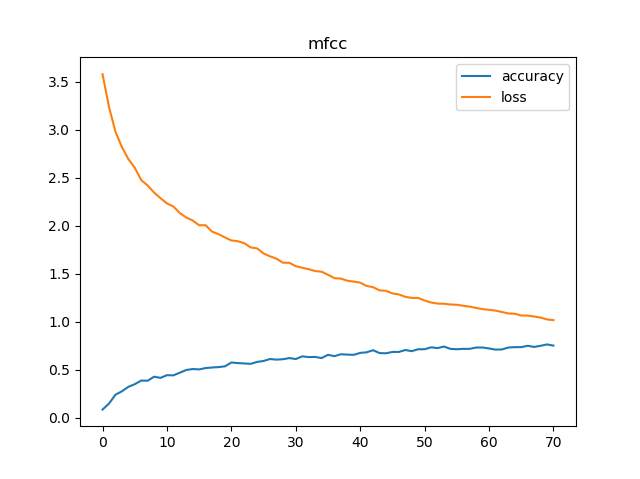
\includegraphics[width=\textwidth]{./graph/mfcc.png} 
\caption{MFCC Training Accuracy and Loss}
\label{mfcc_result}
\end{minipage}
\begin{minipage}[t]{0.5\textwidth}
\centering
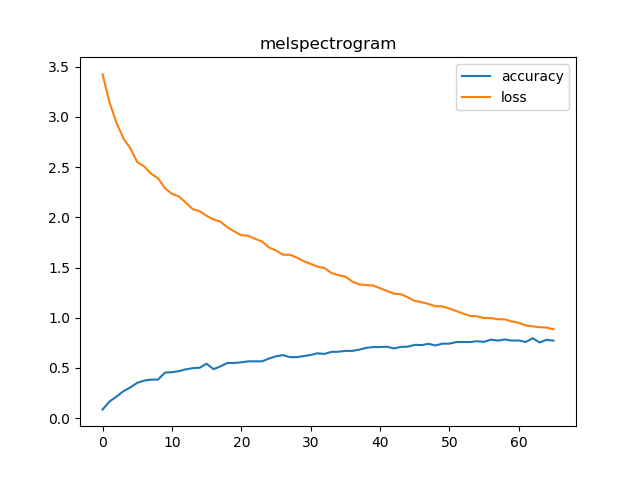
\includegraphics[width=\textwidth]{./graph/melspectogram_result.png} 
\caption{Mel-Spectrogram Training Accuracy and Loss}
\label{sp_result}
\end{minipage}
\end{figure}